\documentclass[parskip=full]{scrartcl}

\pdfoutput=1

\title{Tabular synthetic data generation: A literature review}

\author{%
	Joao Fonseca\(^{1*}\), Fernando Bacao\(^{1}\)
	\\
	\small{\(^{1}\)NOVA Information Management School, Universidade Nova de Lisboa}
	\\
	\small{*Corresponding Author}
	\\
	\\
	\small{Postal Address: NOVA Information Management School, Campus de
    Campolide, 1070--312 Lisboa, Portugal}
	\\
	\small{Telephone: +351 21 382 8610}
}

\usepackage{float}
\usepackage{graphicx}
\usepackage{geometry}
\geometry{%
	a4paper,
	left=18mm,
	right=18mm,
	top=18mm,
}
\usepackage{amsmath}
\usepackage{amsfonts}
\usepackage{enumitem}
\usepackage[ruled,vlined]{algorithm2e}
\usepackage{booktabs}
\usepackage{pgfplotstable}
\pgfplotsset{compat=1.14}
\usepackage{longtable}
\usepackage{tabu}
\usepackage{hyperref}
\usepackage{lineno}
\date{}


% use \citet for inline text references, \cite for normal citations
\usepackage[
    style=numeric,
    citestyle=numeric,
    sorting=none,
    natbib=true,
    backend=biber, 
    maxcitenames=1, 
    maxbibnames=99
]{biblatex}
\bibliography{references}
\usepackage{breakcites}

% Fix underfull hbox warnings in bilbliography
% Reference: https://tex.stackexchange.com/questions/10924/underfull-hbox-in-bibliography
\usepackage{etoolbox}
\apptocmd{\sloppy}{%
    \hbadness%
    10000\relax
}{}{}

% Fix overfull hbox warnings in bibliography
% Reference: https://tex.stackexchange.com/questions/171999/overfull-hbox-in-biblatex
\usepackage[T1]{fontenc}
\usepackage[final]{microtype}

% Highlight text: \hl
\usepackage{soul}

\definecolor{hypecol}{HTML}{0875b7}
\hypersetup{%
    colorlinks,
    linkcolor={hypecol},
    citecolor={hypecol},
    urlcolor={hypecol}
}

% Case-dependent packages here
\usepackage{tabularx}
\renewcommand\tabularxcolumn[1]{m{#1}}% for vertical centering text in X column

\begin{document}

\maketitle
\linenumbers

\begin{abstract}

    The generation of synthetic data can be used for anonymization,
    regularization, oversampling, semi-supervised learning, self-supervised
    learning and various other tasks. The wide range of applications of these
    mechanisms motivated the development of new algorithms specialized in
    generating data for specific types of data and Machine Learning (ML)
    tasks. As a result, the analysis of the different types of generative
    models 

    % We provide a broad taxonomy to define data generation mechanisms

    % We provide an analysis on recommendations for the evaluation of the
    % quality of the synthetic data generated

\end{abstract}

\section{Introduction}~\label{sec:introduction}

Synthetic data is obtained from a generative process based on properties of
real data~\cite{assefa2020generating}. The generation of synthetic data is
essential for various domains and tasks. For example, synthetic data is used
as a form of regularizing neural networks (\textit{i.e.}, data augmentation)
\textbf{[CITATION]}. One form of anonymizing datasets is via the production of
synthetic observations (\textit{i.e.}, synthetic data generation)
\textbf{[CITATION]}. In settings where only a small portion of training data
is labeled, some techniques generate artificial data using both labeled and
unlabeled data with a modified loss function to train neural networks
(\textit{i.e.}, semi-supervised learning)~\cite{laine2017temporal}. In
imbalanced learning contexts, synthetic data can be used to balance the target
classes' frequencies and reinforce the learning of minority classes
(\textit{i.e.}, oversampling)~\cite{fonseca2021improving}. Some active
learning frameworks use data generation to improve the quality of data
selection and classifier training~\cite{kim2021lada}. Other techniques employ
data generation to produce deep neural networks without labeled data
(\textit{i.e.}, self-supervised learning)~\cite{grill2020bootstrap}.

The breadth of these techniques span multiple domains, such as facial
recognition~\cite{lv2017data}, Land Use/Land Cover mapping
\textbf{[CITATION]}, medical image processing \textbf{[CITATION]}, Natural
Language Processing (NLP)~\cite{feng2021survey} or credit card default
prediction~\cite{alam2020investigation}. According to the domain and data
type, the data generation techniques used may vary significantly. Generally
speaking, some data generation mechanisms are specific to some domains, data
types or tasks. \hl{For example, \ldots}. Most, if not all, of these
techniques are applied on the input or output space.

However, there are various data generation techniques that are invariant to
the task or data types used. These techniques can be either applied in the
feature space~\cite{devries2017dataset} or in tabular datasets. On the one
hand, data generation in the feature space uses a generative model to learn a
manifold, lower-dimensional abstraction over the input
space~\cite{kingma2019introduction}, defined here as the feature space. At
this level, any tabular data generation mechanism can be applied and
reconstructed into the input space if necessary. On the other hand, synthetic
data generation on tabular data can be applied to most problems. Although, the
choice of generation mechanism is still dependant on (1) the importance of the
relationships found between the different features, (2) the ML task developed
and (3) the motivation for the generation of synthetic data. For example, when
generating data to address an imbalanced learning problem (\textit{i.e.},
oversampling), the relationships between the different features are not
necessarily kept since the goal is to reinforce the learning of the minority
class by redefining an ML classifier's decision boundaries. If the goal is to
anonymize a dataset, perform some type of descriptive task, or ensure a
consistent model interpretability, these relationships need to be kept.

Depending on the context, evaluating the quality of the generated data is a
complex task. For example, for image and time series data, perceptually small
changes in the original data can lead to large changes in the euclidean
distance~\cite{assefa2020generating, theis2016note}. The evaluation of
generative models typically account primarily for the performance in a
specific task, since good performance in one criterion does not imply good
performance on another~\cite{theis2016note}. However, in computationally
intensive tasks it is often impracticable to search for the optimal
configurations of generative models. To address this limitation, other
evaluation methods have been proposed to assist in this evaluation, which can
be distinguished into statistical divergence metrics and precision/recall
metrics~\cite{alaa2022faithful}. The relevant performance metrics found in the
literature are discussed in Section~\ref{sec:evaluating-synthetic-data}.

% Discuss Generative models -> Network based models

\subsection{Motivation, Scope and Contributions}

% TODO: Define scope
% - Exclude domain-specific traditional applications
% - Exclude Generation techniques with an internal application level
% - Preference for methods published in 2019 or later, or seminal
%   non-traditional methods
% - 

This literatrue review focuses on generation mechanisms applied to tabular
data and the different ML techniques where tabular synthetic data is used. In
addition, we focus on the ML perspective of synthetic data, as opposed to the
practical perspective. From a practical sense, synthetic data is used as a
proxy of real data. It is assumed to be inaccessible, essential and a
secondary asset for tasks like education, software development, or systems
demonstrations~\cite{mannino2019real}. 

We focus on data generation techniques in the tabular and feature space
(\textit{i.e.}, embedded inputs), given its breadth in scope. Related
literature reviews are mostly focused on specific algorithmic or domain
applications, with little to no emphasis on the core generative process. For
this reason, these techniques often appear ``sandboxed'', even though there is
a significant overlap between them. There are some related reviews published
since 2019. \citet{assefa2020generating} provides a general overview of
synthetic data generation for time series data anonymization in the finance
sector. \citet{hernandez2022synthetic} reviews data generation techniques for
tabular health records anonymization. \citet{raghunathan2021synthetic} reviews
synthetic data anonymization techniques that preserve the statistical
properties of a dataset. \citet{nalepa2019data} reviews data augmentation
techniques for brain-tumor segmentation. \citet{bayer2021survey} distinguishes
augmentation techniques for text classification into feature and data space,
while providing an extensive overview of augmentation methods within this
domain. However, the taxonomy proposed and feature space augmentation methods
are not necessarily specific to the domain. \citet{shorten2021text},
\citet{chen2021empirical}, \citet{feng2021survey} and \citet{liu2020survey}
also review data augmentation techniques for text data.
\citet{yi2019generative} review Generative Adversarial Network architectures
for medical imaging. \citet{wang2020survey} reviews face data augmentation
techniques. \citet{shorten2019survey} and \citet{khosla2020enhancing} discuss
techniques for image data augmentation. \citet{iwana2021empirical} and
\citet{wen2020time} also review time series data augmentation techniques.
\citet{zhao2022graph} review data augmentation techniques for graph data. The
analysis of related literature reviews~\footnote{%
    Results obtained using Google Scholar, limited to articles published since
    2019, using the search query {\fontfamily{qcr}\selectfont (``synthetic
    data generation'' OR ``oversampling'' OR ``imbalanced learning'' OR ``data
    augmentation'') AND (``literature review'' OR ``survey'')}. Retrieved on
    August $11^{th}$, 2022. More articles were added later whenever found
    relevant.
} is shown in Table~\ref{tab:literature-reviews}.

% TODO: move table to appendix (?)
\begin{table}[t!]
    \centering
    \caption{\label{tab:literature-reviews}
        Related literature reviews published since 2019.
    }
    \small{
    \begin{tabularx}{\textwidth}{@{}rcccX@{}}
        \toprule
        Reference & Data type & ML problem & Domain & Observations \\
        \midrule

        \citet{assefa2020generating} & --- & Differential privacy &
        Finance & Analysis of applications, motivation and properties of
        synthetic data for anonymization. \\

        \citet{hernandez2022synthetic} & Tabular & Differential privacy &
        Healthcare & Focus on GANs. \\

        \citet{raghunathan2021synthetic} & Tabular & Differential privacy &
        Statistics & Focus on general definitions such as differential privacy
        and statistical disclosure control.\\

        \citet{nalepa2019data} & Image & Segmentation & Medicine & Analysis of
        algorithmic applications on a 2018 brain-tumor segmentation
        challenge.\\

        \citet{bayer2021survey} & Text & Classification & --- & Distinguish
        100 methods into 12 groups. \\

        \citet{shorten2021text} & Text & Deep Learning & --- & General
        overview of text data augmentation. \\

        \citet{chen2021empirical} & Text & Few-shot Learning & --- &
        Augmentation techniques for machine learning with limited data\\

        \citet{feng2021survey} & Text & --- & --- & Overview of augmentation
        techniques and applications on NLP tasks.\\

        \citet{liu2020survey} & Text & --- & Various & Analysis of industry
        use cases of data augmentation in NLP\@. Emphasis on input level data
        augmentation.\\

        \citet{yi2019generative} & Image & --- & Medicine & Emphasis on GANs.\\

        \citet{wang2020survey} & Image & Deep Learning & --- & Regularization
        techniques using facial image data. Emphasis on Deep Learning
        generative models.\\

        \citet{shorten2019survey} & Image & Deep Learning & --- & Emphasis on
        data augmentation as a regularization technique.\\

        \citet{khosla2020enhancing} & Image & --- & --- & Broad overview of
        image data augmentation. Emphasis on traditional approaches. \\

        \citet{iwana2021empirical} & Time series & Classification & --- &
        Defined a taxonomy for time series data augmentation.\\

        \citet{wen2020time} & Time series & Various & --- & Analysis of data
        augmentation methods for classification, anomaly detection and
        forecasting.\\

        \citet{zhao2022graph} & Graph & Various & --- & Graph data
        augmentation for supervised and self-supervised learning.\\

        \citet{khalifa2021comprehensive} & Image & --- & Various & General
        overview of image data augmentation and relevant domains of
        application.\\

        \bottomrule
        
    \end{tabularx}
    }
\end{table}


The different taxonomies established in the literature follow a similar
philosophy, but vary in terminology and are often specific to the technique
discussed. Regardless, it is possible to establish a broader taxonomy without
giving up on specificity. This study provides a joint overview of the
different data generation approaches, domains and ML techniques where data
generation is being used, as well as a common taxonomy across domains. It
extends the analyses found in these articles and uses the compiled knowledge
to identify research gaps. We compare the strengths and weaknesses of the
models developed within each of these fields. Finally, we identify possible
future research directions to address some of the limitations found. The
contributions of this paper are summarized below:

\begin{itemize}
    \item Bridge different ML concepts using synthetic data generation in its
        core \hl{(Algorithmic applications + Review of the State-of-the-art)}.
    \item Propose a synthetic data generation/data augmentation taxonomy to
        resolve the ambiguity in the literature \hl{(Data augmentation
        taxonomy)}.
    \item Characterize all relevant data generation methods using the proposed
        taxonomy. 
    \item Discuss the ML techniques in which synthetic data generation/data
        augmentation is used, beyond regularization and consolidate the
        current data generation mechanisms across the different techniques
        \hl{(Algorithmic Applications)}.
    \item Bring to light the key challenges of synthetic data generation and
        put forward possible research directions in the future.
\end{itemize}

% TODO: Develop research questions

\subsection{Paper Organization}

This paper is organized as follows: Section~\ref{sec:background} defines and
formalizes the different concepts, goals, trade-offs and motivations related
to synthetic data generation. Section~\ref{sec:taxonomy} establishes the
taxonomy used to categorize all the methods described in the paper.
Section~\ref{sec:feature-space} reviews synthetic data generation
mechanisms in the feature space. Section~\ref{sec:input-space}
reviews synthetic data generation mechanisms in the input space.
Section~\ref{sec:algorithmic-applications} describes the applications of
synthetic data in ML methods. Section~\ref{sec:evaluating-synthetic-data}
reviews performance evaluation methods of synthetic data generation
mechanisms. Section~\ref{sec:discussion} summarizes the main findings and
discusses limitations and possible research directions in the
state-of-the-art. Section~\ref{sec:conclusions} presents the main conclusions
drawn from this study.

\section{Background}~\label{sec:background}

% Definition
In this section we define basics concepts, common goals, trade-offs and
motivations regarding the generation of synthetic data in ML\@. We define
synthetic data generation as the production of observations using a generative
model (regardless of its nature) that resemble naturally occurring
observations within a certain domain. It requires access to either a training
dataset, a generative process, or a data stream. However, additional
requirements might be imposed depending on the ML task being developed. For
example, to generate artificial data for regularization purposes in supervised
learning (\textit{i.e.}, data augmentation) the training dataset must be
annotated \textbf{[CITATION]}. The generation of synthetic data for
anonymization purposes assumes synthetic datasets to be different from the
original data, while following the same statistical properties
\textbf{[CITATION]}. Domain knowledge may also be necessary to encode specific
relationships among features into the generative process.


\subsection{Use Cases}

%% Anonymize datasets (differential privacy)
The breach of sensitive information is an important barrier to the sharing of
datasets, especially when it concerns personal
information~\cite{dankar2021fake}. A common solution for this problem is the
generation of synthetic data without identifiable information. Generally
speaking, ML tasks that require data with sensitive information are not
compromised when using synthetic data.  The experiment conducted by
\citet{patki2016synthetic} using relational datasets showed that in 11 out 15
comparisons ($\approx 73\%$), practitioners performing predictive modelling
tasks using fully synthetic datasets performed the same or better than those
using the original dataset. This topic is discussed in
Section~\ref{sec:data-privacy}.

%% Generalization/regularization
A common problem in the training of deep neural networks are their capacity to
generalize~\cite{Zhang2021} (\textit{i.e.}, reduce the difference in
classification performance between known and unseen observations). Data
augmentation is a common method to address this problem. The generation of
synthetic observations increases the range of the possible input space used in
the training phase, which reduces the performance difference between known and
unseen observations. Although other regularization methods exist, data
augmentation is a useful method since it does not affect the choice in the
architecture of the ML classifier and does not exclude the usage of other
regularization methods. In domains such as computer vision and NLP, data
augmentation is also used to improve the robustness of models against
adversarial attacks~\cite{zeng2020data, morris2020textattack}. These topics
are discussed into higher detail in Section~\ref{sec:regularization}.

%% Oversampling
In supervised learning, synthetic data generation is often motivated by the
need to balance target class distributions (\textit{i.e.}, oversampling).
Since most ML classifiers are designed to perform best with balanced datasets,
defining an appropriate decision boundary to distinguish rare classes becomes
difficult~\cite{saez2016analyzing}. Although there are other approaches to
address imbalanced learning, oversampling techniques are generally easier to
implement since they do not involve modifications to the classifier. This
topic is discussed into higher detail in Section~\ref{sec:oversampling}.

%% Active Learning + Few-shot Learning
In supervised learning projects where labeled data is not readily available,
but can be labeled, an Active Learning (AL) method may be used to improve the
labelling process. AL aims to reduce the cost of producing training datasets
by finding the most informative observations to label and feed into the
classifier~\cite{fonseca2021increasing}. In this case, the generation of
synthetic data is particularly useful to reduce the amount of labelled data
required for a successful ML project and its costs. A similar motivation
applies to the case of few-shot learning: small datasets may be expanded with
synthetic data~\cite{kumar2019closer}. These topics are discussed in
Sections~\ref{sec:active-learning} and~\ref{sec:few-shot-learning}.

%% Semi-supervised Learning + Self-supervised learning
The two other techniques reliant on synthetic data generation is 
Semi-supervised and Self-supervised learning. The former leverages both
labeled and unlabeled data in the training phase, simultaneously. Most of the
methods in the literature apply perturbations on the training data as part of
the training procedure~\cite{van2020survey}. Self-supervised learning is a
technique used to train neural networks in the absence of labeled data. Both
techniques use synthetic data generation as an internal procedure for most of
these methods. These techniques are discussed in
Sections~\ref{sec:semi-supervised-learning}
and~\ref{sec:self-supervised-learning}.


% Concepts definition, goals + trade-offs, Motivations

% Concepts definition
% - Original dataset
% - Synthetic dataset
% - Generator
% - Quality criteria (e.g., similarity function)
% - Objective performance metric (ML method to improve)
 
% Common success criteria 
% - The synthetic dataset should be different than the original dataset (i.e.,
%   no duplicates)
% - It should minimize a similarity function
% - The statistical properties of the dataset are preserved
% - It should improve the output of the objective performance
 
% Trade-offs
% - Additional computational overhead
% - Expose the classifier to unfeasible input areas

\subsection{Problem Formulation}~\label{sec:problem-formulation}

The original dataset, $\mathcal{D} = \mathcal{D}_L \cup \mathcal{D}_U$,
is a collection of real observations and is distinguished according to whether
a target feature exists, $\mathcal{D}_L = {((x_i, y_i))}^l_{i=1}$, or not,
$\mathcal{D}_U = {(x_i)}^{u}_{i=1}$. All three datasets, $\mathcal{D}$,
$\mathcal{D}_L$ and $\mathcal{D}_U$ consist of ordered collections with
lengths $l+u$, $l$ and $u$, respectively. Synthetic data generation is
performed using a generator, $f_{gen}(x;\tau) = \tilde{x}$, where $\tau$
defines the generation policy (\textit{i.e.}, its hyperparameters), $x \in
\mathcal{D}$ is an observation and $\tilde{x} \in \mathcal{D}^s$ is a
synthetic observation. Analogous to $\mathcal{D}$, the synthetic dataset,
$\mathcal{D}^s$, is also distinguished according to whether there is an
assignment of a target feature, $\mathcal{D}^s_L = {((\tilde{x}_j,
\tilde{y}_j))}^{l'}_{j=1}$, or not, $\mathcal{D}^s_U =
{(\tilde{x}_j)}^{u'}_{j=1}$.

% - Quality criteria (e.g., similarity function)
Depending on the ML task, it may be relevant to establish metrics to measure
the quality of $\mathcal{D}^s$. In this case, a metric
$f_{qual}(\mathcal{D}^s, \mathcal{D})$ is used to determine the level of
similarity/dissimilarity between $\mathcal{D}$ and $\mathcal{D}^s$. In
addition, a performance metric to estimate the performance of a model on the
objective task, $f_{per}$, may be used to determine the appropriateness of a
model with parameters $\theta$, \textit{i.e.}, $f_{\theta}$. The generator's
goal is to generate $\mathcal{D}^s$ with arbitrary length, given
$\mathcal{D} \sim \mathbb{P}$ and $\mathcal{D}^s \sim \mathbb{P}^s$, such
that $\mathbb{P}^s \approx \mathbb{P}$, $x_i \neq x_j \forall x_i \in
\mathcal{D} \wedge x_j \in \mathcal{D}^s$. $f_{gen}(x;\tau)$ attempts to
generate a $\mathcal{D}^s$ that maximizes either $f_{per}$, $f_{qual}$, or a
combination of both.


\section{Data Generation Taxonomy}~\label{sec:taxonomy}

The taxonomy proposed in this paper is a compilation of different definitions
found in the literature, along with other traits that vary among domains and
generation techniques. Within image data studies, \citet{shorten2019survey}
and \citet{khalifa2021comprehensive} divide data augmentation techniques into
``basic'' or ``classical'' approaches and deep learning approaches. In both
cases, the former refers to domain-specific generation techniques, while the
latter may be applied to any type of data. \citet{iwana2021empirical} proposes
a time-series data augmentation taxonomy divided in four families: (1)
Decomposition, (2) Pattern mixing, (3) Generative models and (4)
Decomposition. With exception to generative models, the majority of the
methods presented in the remaining families are well established and domain
specific. \citet{hernandez2022synthetic} defines a taxonomy for synthetic
tabular data generation approaches divided in three types of approaches: (1)
Classical, (2) Deep learning and (3) Others.  Most taxonomies found followed
similar definitions with variations in terminology or distinction criteria. In
addition, all taxonomies with categories defined as ``basic'', ``traditional''
or ``classical'' use these to characterize domain-specific transformations.




Within the taxonomies considered, none of them consider how a generation
mechanism employs $\mathcal{D}$ into the generation process or, if
applicable, the training phase. However, it is important to understand whether
a generation mechanism randomly selects $x$ and a set of close neighbors, thus
considering local information only, or considers the overall dataset or data
distribution for the selection of $x$ and/or generation of $\tilde{x}$. Our
proposed taxonomy is depicted in Figure~\ref{fig:data-generation-taxonomy}. It
characterizes data generation mechanisms using four properties:

\begin{enumerate}

    \item Architecture. Defines the broader type of data augmentation. It is
        based on domain specificity, architecture type or data transformations
        using a heuristic or random perturbation process. Generation
        techniques that apply a form of random perturbation, interpolation or
        geometric transformation to the data with some degree of randomness
        are considered randomized approaches. Typical, domain-specific data
        generation techniques are considered traditional architectures. These
        techniques apply transformations to a data point using \textit{a
        priori} domain knowledge. Generative models based on neural network
        architectures are defined as network-based. These architectures
        attempt to either generate observations in the feature space and/or by
        producing observations that are difficult to distinguish from the
        original dataset.

    \item Application level. Refers to the phase of the ML pipeline where the
        generative process is included. Generative models are considered
        internal if they are used alongside the primary ML task, whereas
        models used prior to the development of the primary ML task are
        considered external.

    \item Scope. Considers the usage of the original dataset's properties.
        Generative models that consider the density of the data space,
        statistical properties of $\mathcal{D}$, or attempt to replicate
        specific relationships found in $\mathcal{D}$ are considered to have
        a global scope, whereas generative models that consider a single
        observation and/or a set of close neighbors are considered to have a
        local scope. On the one hand, generative models with a local scope do
        not account for $\mathbb{P}^s$ but allow for a larger diversity of
        candidate $x^s$ and higher variance within $\mathcal{D}^s$. On the
        other hand, generative models with a global scope have a higher
        capacity to model $\mathbb{P}^s$ but produce candidate $x^s$ with
        lower diversity and lower variance within $\mathcal{D}^s$.

    \item Data space. Refers to the type data representation used to apply the
        generative model. Generation mechanisms can be applied using the raw
        dataset (\textit{i.e.}, on the input space), an embedded
        representation of the data (\textit{i.e.}, on the feature space) or
        based on the target feature (\textit{i.e.}, on the output space).

\end{enumerate}

\begin{figure}
	\centering
	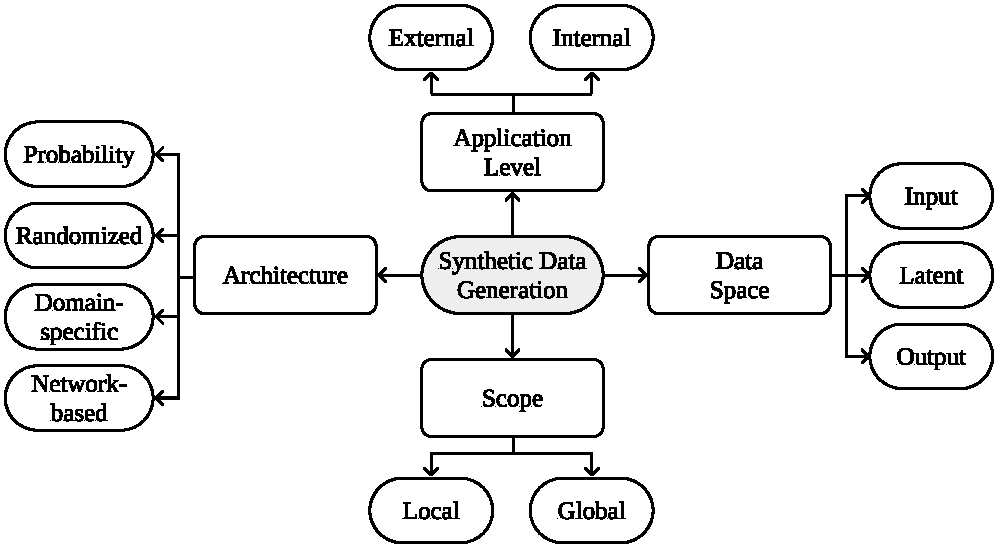
\includegraphics[width=.8\linewidth]{../analysis/data-generation-taxonomy}
    \caption{General taxonomy of data generation mechanisms proposed in this
        paper.
    }~\label{fig:data-generation-taxonomy}
\end{figure}

Throughout the analysis of the different types of generation mechanisms, all
relevant methods were characterized using this taxonomy and listed in
Table~\ref{tbl:generators}.

\begingroup\small
\begin{longtable}{rcccccccc}
    \caption{Summary of synthetic data generation mechanisms discussed in this work.}
    \label{tbl:generators}\\
    \toprule
               Algorithm & ML problem & Domain &  Architecture & Level &  Data
               Space & Scope \\
    \midrule
    \endfirsthead
    \caption[]{Summary of synthetic data generation mechanisms discussed in this work.} \\
    \toprule
               Algorithm & ML problem & Domain &  Architecture & Level &  Data
               Space & Scope \\
    \midrule
    \endhead
    \midrule
    \multicolumn{9}{r}{{Continued on next page}} \\
    \midrule
    \endfoot
    
    \bottomrule
    \endlastfoot
      SynSys~\cite{dahmen2019synsys} & Reg. & Healthcare & \textbf{[Statistical]}  & External & Input & Global \\
      CTGAN~\cite{xu2019modeling} & & --- & Net. & External & Feature & Global \\
      SenseGen~\cite{alzantot2017sensegen} & Anon. + Reg. & Sensor & Net. + \textbf{[Stat.]} & External & Input & Global\\
      SDV~\cite{patki2016synthetic} & Anon. & --- & \textbf{[Copula]} & External & Input & Global \\
      MST~\cite{mckenna2021winning} & DP & --- & \textbf{[Statistical]} & External & Input & Global \\
      QUAIL~\cite{rosenblatt2020differentially} & DP \\
      SuperQUAIL~\cite{rosenblatt2022spending} & DP \\
      MWEM~\cite{hardt2012simple} & DP \\
      MWEM-PGM~\cite{mckenna2019graphical} & DP \\
      PrivBayes~\cite{zhang2017privbayes} & DP\\
      DPGAN~\cite{xie2018differentially} & DP \\
      DPCTGAN~\cite{rosenblatt2020differentially} & DP & \\
      DP-CTGAN~\cite{fang2022dp} & DP & Healthcare \\
      PATE-GAN~\cite{jordon2018pate} & DP \\
      PATECTGAN~\cite{rosenblatt2020differentially} & DP \\
      FEM~\cite{vietri2020new} & DP \\
      RAP~\cite{aydore2021differentially} & DP \\
      Kamino~\cite{ge2020kamino} & DP \\
      RON-GAUSS~\cite{chanyaswad2019ron} & DP \\
      SMOTE~\cite{chawla2002smote} & Ovs \\
      SMOTENC~\cite{chawla2002smote} & Ovs \\
      SMOTEN~\cite{chawla2002smote} & Ovs \\
      Borderline-SMOTE~\cite{han2005borderline} & Ovs \\
      G-SMOTE~\cite{douzas2019geometric} & Ovs \\
      ADASYN~\cite{he2008adasyn} & Ovs \\
      KernelADASYN~\cite{tang2015kerneladasyn} & Ovs \\
      Safe-level SMOTE~\cite{bunkhumpornpat2009safe} & Ovs \\
      LR-SMOTE~\cite{liang2020lr} & Ovs \\
      K-means SMOTE~\cite{douzas2018improving} & Ovs \\
      CGAN~\cite{douzas2018effective} & Ovs \\
      K-means CTGAN~\cite{an2021k} & Ovs \\
      G-SMOTER~\cite{camacho2022geometric} & Ovs + Reg \\
      SMOTER~\cite{torgo2013smote} & Ovs + Reg \\
\end{longtable}
\endgroup


% \section{Data Generation in the Input Space}~\label{sec:input-space}
% 
% In this section, we describe some popular domain and data type-specific data
% generation techniques. For each data type we include a table with related
% literature reviews specific to different domains.
% 
% \subsection{Supervised data generation}
% % TODO: 
% % - Table with literature review references 
% 
% \subsection{Unsupervised data generation}
% % TODO: 
% % - Table with literature review references 

% \subsection{Image}
% % TODO: 
% % - Table with literature review references 
% 
% Image-specific data generation mechanisms can be further divided into
% traditional and semantic techniques~\cite{wang2021regularizing}. Traditional
% generation techniques comprise simple modifications such as translation,
% cropping or random erasing~\cite{zhong2017random}. Semantic generation methods
% involve more complex tasks, such changing colors of specific attributes,
% backgrounds and visual angles \textbf{[CITATION]}. 
% % Go back to explaining wang2021regularizing
% 
% % semantic generation technique
% Data generation by modifying specific attributes in data points with known
% perturbations~\cite{lv2017data}. For example, overlaying facial elements into
% a picture containing a human face (\textit{e.g.}, adding sunglasses and
% different hairstyles), introducing perturbations in facial landmarks,
% different illumination and artificial misalignment are different approaches to
% generate artificial observations for facial recognition.
% 
% % GANs
% Generative Adversarial Networks in computer vision~\cite{wang2021generative}

% traditional
% - mixup

% \subsection{Text}
% % TODO: 
% % - Table with literature review references 
% 
% NLP motivations~\cite{feng2021survey}:
% 
% \begin{enumerate}
%     \item Low-resource languages (NLP)
%     \item Mitigate bias
%     \item Fixing class imbalance
%     \item Few-shot learning
%     \item Adversarial examples
% \end{enumerate}
% 
% 
% NLP also benefit from data augmentation~\cite{feng2021survey}.
% 
% In NLP, there is the challenge of establishing universal rules for text
% transformations to provide new linguistic patterns~\cite{bayer2022data}
% 
% https://github.com/styfeng/DataAug4NLP
% 
% \subsection{Graphs}
% 
% 
% Another relevant paper~\cite{zhou2020data}
% 
% Various graph data augmentation methods can be applied to related data types
% such as text data~\cite{shorten2021text}.
% 
% 
% An analysis on different graph data augmentation techniques and a new graph
% data augmentation framework~\citet{zhao2021data}
% 
% List of papers about graph data augmentation:
% https://github.com/zhao-tong/graph-data-augmentation-papers




% \section{Data Generation in the Feature Space}~\label{sec:feature-space}
% % Feature level data augmentation
% 
% The concept of data generation in the feature space was popularized
% with~\cite{devries2017dataset}.
% 
% According to~\cite{assefa2020generating}. The generation of synthetic data
% should aim to fulfil the conditions below:
% 
% \begin{itemize}
%     \item Privacy preserving.
%     \item Human readable.
%     \item Compact.
% \end{itemize}
% 
% Discuss Auto-augmentation (as mentioned in~\cite{wang2020survey}) or meta
% learning (as mentioned in~\cite{shorten2019survey})


\section{Algorithmic applications}~\label{sec:algorithmic-applications}

In this section we discuss the data generation mechanisms for the different
contexts where they are applied. We emphasize the constraints in each problem
that condition the way generation mechanisms are used.

CTGAN~\cite{xu2019modeling}

\subsection{Dataset Anonymization}~\label{sec:data-privacy}

% Introduce synthetic data generation
Synthetic data generation is a technique used to produce synthetic, anonymized
versions of datasets~\cite{dankar2021fake}. It is considered a good approach
to share sensitive data without compromising significantly a given data mining
task~\cite{taub2018differential, park2018data}. Traditional data anonymization
techniques, as well as federated learning are two other viable solutions for
privacy-preserving data publishing tasks, but contain
drawbacks~\cite{hernandez2022synthetic}. On the one hand, traditional data
anonymization requires domain knowledge, is labor intensive and remains
susceptible to disclosure~\cite{reiter2004new}. On the other hand, federated
learning is a technically complex task that consists on training ML
classifiers on edge devices and aggregating temporarily updated parameters on
a centralized server, instead of aggregating the training
data~\cite{yu2022survey}. Although it prevents sharing sensitive data, its
applicability is dependent on the task. Dataset anonymization via synthetic
data generation attempts to balance disclosure risk and data utility in the
final synthetic dataset. The goal is to ensure observations are not
identifiable and the relevant data mining tasks are not
compromised~\cite{singh2017aggregating, li2018privacy}.

The generation of synthetic datasets allow a more flexible approach to the
successful implementation of ML tasks. To do this, it is important to
guarantee that sensitive information in $\mathcal{D}$ is not leaked into
$\mathcal{D}^s$. Differential privacy (DP), a formalization of privacy, offers
strict theoretical privacy guarantees~\cite{rosenblatt2020differentially}. A
differentially private generation mechanism produces a synthetic dataset,
regulated by the privacy parameter $\epsilon$, with statistically
indistinguishable results when using either $\mathcal{D}$ or neighboring
datasets $\mathcal{D}' = \mathcal{D} \backslash \{x\}$, for any $x \in
\mathcal{D}$. A synthetic data generation model ($f_{gen}$) guarantees
$(\epsilon, \delta)$-differential privacy if $\forall S \subseteq
Range(f_{gen})$ all $\mathcal{D}, \mathcal{D}'$ differing on a single
entry~\cite{hardt2012simple}:

\begin{equation}
    Pr[f_{gen}(\mathcal{D}) \in S] \le e^{\epsilon} \cdot
    Pr[f_{gen}(\mathcal{D}') \in S] + \delta
\end{equation}
 
In this case, $\epsilon$ is a non-negative number defined as the privacy
budget. A lower $\epsilon$ guarantees a higher level of privacy, but reduces
the quality of the produced synthetic data. The generation of DP synthetic
data is especially appealing since DP is not affected by post-processing; any
ML pipeline may be applied using $\mathcal{D}^s$ without a loss of
differential privacy.

Despite the formalization and the ability to quantify differential privacy,
there are popular synthetic data-based anonymization approaches that perform
this task without DP guarantees. Specifically, the Synthetic Data Vault
(SDV)~\cite{patki2016synthetic} is a method for database anonymization that
uses Gaussian Copula models for generating data. However, this method allows
the usage of other generation mechanisms. A posterior extension of SDV was
proposed to generate data using a CTGAN~\cite{xu2019modeling} and to handle
sequential tabular data using a conditional probabilistic auto-regressive
neural network~\cite{zhang2022sequential}. 

The MST mechanism~\cite{mckenna2021winning} is a general approach that
produces differentially private data. It uses the Private-PGM
mechanism~\cite{mckenna2019graphical} that relies on Probabilistic Graphical
Models (PGM) to generate synthetic data. PGM models are most commonly used
when it is important to maintain the pre-existing relationships between
features and statistical properties in $\mathcal{D}$~\cite{young2009using}.

Anonymizing data using synthetic data generation in the financial
sector~\cite{assefa2020generating}.


A benchmark of various differentially private synthetic data generation
mechanisms~\cite{tao2021benchmarking}.


Guidelines for effective synthetic data generation~\cite{dankar2021fake}





\subsection{Regularization in Supervised Learning}~\label{sec:regularization}

% Introduce data augmentation
The performance of Machine Learning models is highly dependent on the quality
of the training dataset used~\cite{Fenza2021, Halevy2009}. The presence of
imbalanced and/or small datasets, target labels incorrectly assigned, outliers
and high dimensional input spaces reduce the prospects of a successful machine
learning (ML) model implementation~\cite{Halevy2009, Domingos2012,
Salman2019}. In the case of deep learning, for example, these
models are often limited by a natural inclination to overfitting, label noise
memorization and catastrophic forgetting~\cite{Xie2021}. Regularization
methods are the typical approach to address these problems, but producing
robust ML solutions is still a challenge~\cite{Zhang2021}.

It is frequently assumed that the training data is sampled from a fixed data
source, it is balanced and does not contain label noise. Under these
conditions, the resulting ML classifier is expected to achieve good
generalization performance~\cite{benning2018modern}. Although, in practical
applications, this is rarely the case. When the training data is not
representative of the true population, or the model is over-parametrized, it
becomes particularly prone to overfitting~\cite{Bartlett2021}. Regularization
methods attempt to address these limitations. They can be divided into three
categories~\cite{santos2022avoiding}:

\begin{enumerate}
    \item Output level modifications. Transforms the labels in the training
        data.
    \item Algorithmic level modifications. Modifies the classifier's
        architecture, loss function or other components in the training
        procedure.
    \item Input level modifications. Modifies the training dataset by expanding it
        with synthetic data.
\end{enumerate}

The last approach, input level modifications, is known as data augmentation.
Data augmentation is used to increase the size and data variability of data in
a training dataset, by producing synthetic observations~\cite{Van2001,
Wong2016}. Since it is applied at the data level, it can be used for various
types of problems and classifiers~\cite{Behpour2019}. 

Problems such as fraud detection and healthcare are frequently tackled via
synthetic data generation~\cite{ekbatani2017synthetic}.

``Su et al. [78] show that 70.97\% of images can be misclassified by changing
just one pixel'' \citet{shorten2019survey}

``Moreover, the current research about so called adversarial attacks on CNNs
showed that deep neural networks can be easily fooled into misclassification
of images just by partial rotations and image translation [1], adding the
noise to images [5] and even changing one, skillfully selected pixel in the
image [6].'' \citet{mikolajczyk2018data}

Data augmentation can also be used to improve a model's robustness against
adversarial attacks. 

% NOTE: Using an ensemble of views of the same observation to the same
% classifier and checking the different predictions has surely been explored
% (?) 
% i.e., augmentation at inference time, instead of training


\subsection{Time Series}
% TODO: 
% - Table with literature review references 

% A general description of time series data

Synsys~\cite{dahmen2019synsys} approaches time-series using both Hidden Markov
and regression models. They show the method's effectiveness in the Healthcare
domain with limited ground truth data by comparing it to models trained using
only real data. A related model, Sensegen~\cite{alzantot2017sensegen}, uses an
adversarial training approach to train an LSTM that predicts the parameters
of Gaussian Mixture Models (GMM) at each time stamp, using real data as
an input. Finally, the GMM estimations are used to sample synthetic data. 


Generative adversarial networks in time series 


\subsection{Oversampling}~\label{sec:oversampling}

KernelADASYN~\cite{tang2015kerneladasyn}

The original author of SMOTE recently published the paper ``Efficient Augmentation for Imbalanced Deep
Learning''~\cite{dablain2022efficient}

\subsection{Active Learning}~\label{sec:active-learning}

\subsection{Few-shot Learning}~\label{sec:few-shot-learning}

Analysis of six feature space data augmentation techniques for few-shot
learning~\cite{kumar2019closer}

FlipDA~\cite{zhou2021flipda}

Data generation can be used to address Few-shot learning in three
ways~\cite{wang2020generalizing}: (1) transforming samples from the dataset,
(2) transforming samples from a weakly labeled or unlabeled dataset, or (3)
transforming samples from similar datasets.

\subsection{Semi-supervised Learning}~\label{sec:semi-supervised-learning}

Synthetic data generation for semi-supervised learning given limited labeled
data regarding the COVID-19 pandemic~\cite{das2022conditional}.

Extensive literature review on semi-supervised learning~\cite{van2020survey}

\subsection{Self-supervised Learning}~\label{sec:self-supervised-learning}

\section{Evaluating the Quality of Synthetic Data
}~\label{sec:evaluating-synthetic-data}

The log-likelihood (and equivalently the Kullback-Leibler Divergence) is a
de-facto standard to train and evaluate generative
models~\cite{theis2016note}. Other common metrics include Parzen window
estimates, which~\citet{theis2016note} show that these metrics behave
independently and should generally be avoided. Therefore, it is necessary
to evaluate generative models with respect to the application these models are
being developed for.


The evaluation of generative models should quantify three key aspects of
synthetic data~\cite{alaa2022faithful}:

\begin{enumerate}
    \item Fidelity
    \item Diversity 
    \item Generalization
\end{enumerate}

The 3-dimensional metric proposed by~\citet{alaa2022faithful} quantifies these
aspects via the combination of three metrics ($\alpha$-Precision,
$\beta$-Recall and Authenticity) for various application domains.

\subsection{Statistical Divergence Metrics} 

\subsection{Precision/Recall Metrics}

\section{Discussion}~\label{sec:discussion}

\subsection{Main Findings}

The combination of data generation strategies is an approach commonly found in
different problems, such as self-supervised
learning~\cite{grill2020bootstrap}. It can be more frequently found in text
data applications~\cite{bayer2021survey} and image data \textbf{[CITATION]}.

\subsubsection{RQ1: bla bla bla}

\subsubsection{RQ2: bla bla bla}

\subsubsection{RQ3: bla bla bla}

\subsection{Limitations}

Research across the different applications appears to be sandboxed even though
all techniques integrate synthetic data in its core.

Given the breadth and complexity of input-level and feature-level data
generation mechanisms, it is increasingly important to find a method to
efficiently determine the most appropriate data generation policies. However,
the complexity of this task is determined by various factors: different data
types, ML problems, model architectures, computational resources, performance
metrics and contextual constraints. Auto-augmentation and meta learning aim to
address this challenge and are still subject to active research.

% Synthetic data generation with a real valued y?

% data privacy
The evaluation of anonymization techniques lack standardized, objective and
reliable performance metrics and benchmark datasets to allow an easier
comparison across classifiers to evaluate key aspects of data anonymization
(resemblance, utility, privacy and performance). These datasets should contain
mixed data types (\textit{i.e.}, a combination of categorical, ordinal,
continuous and discrete features) and the metrics should evaluate the
performance of different data mining tasks along with the anonymization
reliability. This problem appears to be universal across domains. For example,
\citet{hernandez2022synthetic} observed the lack of a universal method or
metric to report the performance synthetic data generation algorithms for
tabular health records. Therefore, in order to facilitate the usage of these
techniques in industry domains, these benchmarks must also be
realistic. \citet{rosenblatt2020differentially} attempts to address this
problem by proposing a standardized evaluation methodology using standard
datasets and real-world industry applications.

Computational cost and inconsistent quality of synthetic data generated with
GANs (\textit{e.g.}, mode collapse).

% Regularization in supervised learning
Unlike with data privacy solutions, data augmentation techniques generally do
not consider the similarity/dissimilarity of synthetic data. The study of
quality metrics for supervised learning may reduce computational overhead and
experimentation time. No studies related to the relationship of quality
metrics and performance in the primary ML task were found
\textbf{[CONFIRM!!!]}.

There is not a clear understanding of what types of data augmentation methods
are more appropriate according to different model architectures, ML tasks or
domains and the reason why they work better or worse depending on the task. 
In addition, it is still unclear \textit{why} data augmentation works.
Research on this topic lacks depth and fails to address the theoretical
underpinnings~\cite{feng2021survey}.

``Dao et al. (2019) note that ``data augmentation is typically performed in an
ad-hoc manner with little understanding of the underlying theoretical
principles'', and claim the typical explanation of DA as regularization to be
insufficient.''~\cite{feng2021survey}

% oversampling
There is a lack of research on oversampling solutions to generate synthetic
data with mixed data types and datasets with exclusively non metric features.

There is a lack of methods adapted to use categorical features for tabular
data.

There is a paucity of research on the usage of probabilistic-based generation
mechanisms in oversampling.

% Active Learning

% Semi-supervised Learning

% Self-supervised Learning
There is no clear understanding of the most appropriate data augmentation
techniques used to train self-supervised models and how their behavior and
performance varies according to the data generation method used.

% Societal challenges raised by data generation (?)
% Systematic bias

oversampling does not seem to be a relevant source of bias in behavioral
research and does not appear to have an appreciably different effect on
results for directly versus indirectly oversampled
variables~\cite{hauner2014latent}

% Maybe discuss adversarial attacks?

\subsection{Research directions}

% similarities between mixup and SMOTE, and an intermediate solution that can
% be further explored to use the mixup approach on tabular data
% (Geometric-SMOTE selection mechanism)

Quantifying the quality of the generated data:

\begin{enumerate}
    \item Realistic
    \item Similarity
    \item Usefulness (determine purpose and relevant performance metric)
    \item Understand the relationship between the 3 factors
\end{enumerate}

\section{Conclusions}~\label{sec:conclusions}

\printbibliography

\end{document}
